\documentclass{article}
\usepackage[utf8]{inputenc}
\usepackage[spanish]{babel}
\usepackage{listings}
\usepackage{graphicx}
\graphicspath{ {{c:/user/images/}} }
\usepackage{cite}

\begin{document}

\begin{titlepage}
    \begin{center}
        \vspace*{1cm}
            
        \Huge
        \textbf{}
            
        \vspace{0.5cm}
        \LARGE
        Parcial 2 Parte 2
            
        \vspace{1.5cm}
            
        \textbf{Mateo Cardona Correa}
            
        \vfill
            
        \vspace{0.8cm}
            
        \Large
        Despartamento de Ingeniería Electrónica y Telecomunicaciones\\
        Universidad de Antioquia\\
        Medellín\\
        Septiembre de 2021
            
    \end{center}
\end{titlepage}

\tableofcontents
\newpage
\section{Introduccion al Trabajo}\label{intro}
El trabajo aqui presentado se realiza bajo la consideracion de la presentacion de un problema planteado en la normativa de la cotidianidad, presentando un problema tan comun como puede ser el desarrollo de un programa para transformar nociones, conceptos, programas y algoritmos digitales a un ambiente no digital, como puede ser una pantalla o un grupo de luces, en este caso, leds.
\subsection{Analisis del problema}\label{}
Las clases implementadas fueron:\\
-Clase base QImage: Clase implementada en el codigo de QT\\
-Clase base String: Clase implementada en el codigo de QT\\
\subsection{Esquema Base}\label{}
El esquema que se utilizo fue:\\
-Imagen descargada\\
-Submuestreo de la imagen\\
-Transformacion de la imagen mas pequeña en una serie de caracteres\\
-Lectura de los caracteres por un Arduino\\
-Transformacion de los caracteres en señales electricas\\
-De señales electricas a prender un panel de luces Led
\newpage
\section{Modulo de Codigo} \label{contenido}
Aqui se mostrara el codigo implementado en el programa QT
\begin{lstlisting}[language=C++, label=codigo_ejemplo]
#include <iostream>
#include <fstream>
#include <string>
#include <QImage>

using namespace std;

int main(){
    string filename = "imagen.jpg";
    QImage im(filename.c_str());
    im = im.scaled(8,8);
    string R = "{";
    string G = "{";
    string B = "{";

    for(int j = 0; j < 8; j++){
        for(int i = 0; i < 8; i++){
            R += to_string(im.pixelColor(i,j).red());
            G += to_string(im.pixelColor(i,j).green());
            B += to_string(im.pixelColor(i,j).blue());
            if(j == 7 && i == 7){
                R += "}";
                G += "}";
                B += "}";
            }else{
                R += ", ";
                G += ", ";
                B += ", ";
            }
        }
    }

    ofstream fout;
    fout.open("copiar.txt");
    fout << "//Pegue el siguiente codigo en tinkercad" << endl << endl;
    fout << "byte arr[3][64]{" << endl;
    fout << "\t" << R << "," << endl;
    fout << "\t" << G << "," << endl;
    fout << "\t" << B << endl;
    fout << "};" << endl;
    fout.close();

    return 0;
}
\end{lstlisting}
Como se puede ver en el codigo superior, las clases String y Qimage utilizadas (Pertenecientes a las librerias de igual nombre) se utilizan principalmente para:\\
-Cargar la imagen\\
-Escalar la imagen a un tamaño 8x8\\
-Transformar en caracter cada pixel de la imagen\\
-Asignacion de cada pixel de la imagen al sistema RGB\\
\newpage
\subsection{Estructura del circuito}\label{}
\begin{figure}[htb]
\centering
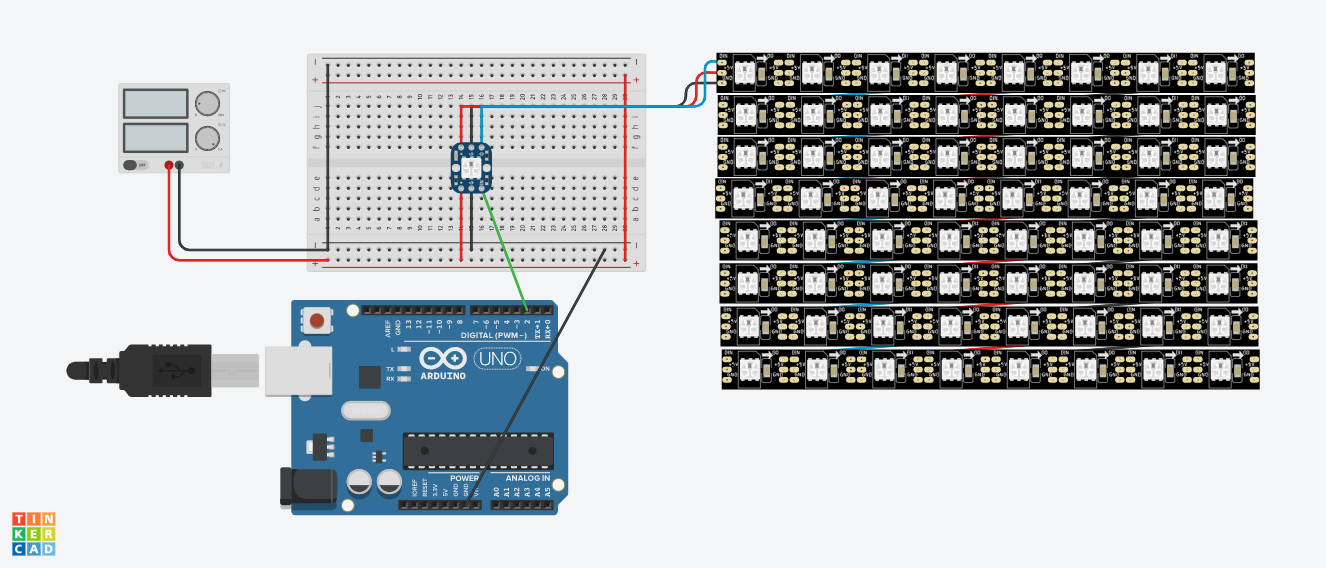
\includegraphics[width=15cm]{Circuito_Parcial_2}
\caption{Circuito utilizado para la exposicion}
\end{figure}
\newpage
\section{Problemas presentados durante el desarrollo}\label{}
Los principales problemas presentados durante el desarrollo fueron:\\
-La utilizacion eficiente del modelo RGB\\
-Guardar la cadena de caracteres en un txt\\
-La composicion propia de la cadena de caracteres\\
-El reescalado de la imagen\\
-La lectura de la cadena de caracteres en un Arduino
\end{document}
